
\subsection{Requirements}

Table 1 presents our requirements by priority level. Our challenge was to develop as many requirements as we could. We are happy as we manage to develop all the first priority  level requirements. However, we must state that we desired to tackle more of the other requirements set in our priorities but for the challenges we encountered as a team.

\begin{table}[ht]
\caption{Requirements by priority level}
\label{tab:requirements}
    \begin{tabular}[c]{ | p{5cm} | p{5cm} | p{5cm} |}
		\hline
		\centering\textbf{Priority 1} & \centering{\textbf{Priority 2}} & \centering\textbf{Priority 3} &
    \hline
    \parbox[t]{5cm}{-Secure connection\\-Encrypted messages\\ -IOS, Android and Web platforms (at least two platforms)\\ -Contact list\\ -Search for contacts\\ -Sign in by email or Gmail \\ -One to one conversation (text message)} &  \parbox[t]{5cm}{-Send images\\ -Group chat\\ -Chat bubbles instead of username\\ -Notifications of received messages}
& \parbox[t]{5cm}{-Sign in by Facebook\\ -Availability to send other type of media (e.g. video, voice notes, etc.)\\ -Online status of other users\\ -Acknowledgement of received, delivered and read messages, including timestamp\\ -Ability to use the chat offline}\\
    \hline
    \end{tabular}
\end{table}


\subsection{Architecture}

In accordance with the definition of Architecture by Eden and Kazman ~\cite{eden2003architecture}, the next Figure  ~\ref{fig:Architecture}  represents the overview of our design. Thus, we implemented three clients, using Firebase as a back-end, and a JSON, NoSQL (non relational) Database designed to make read operations lighting fast, which involved a trade-off, where we prioritise read speed over data normalisation.

\begin{figure}[ht]
\centering
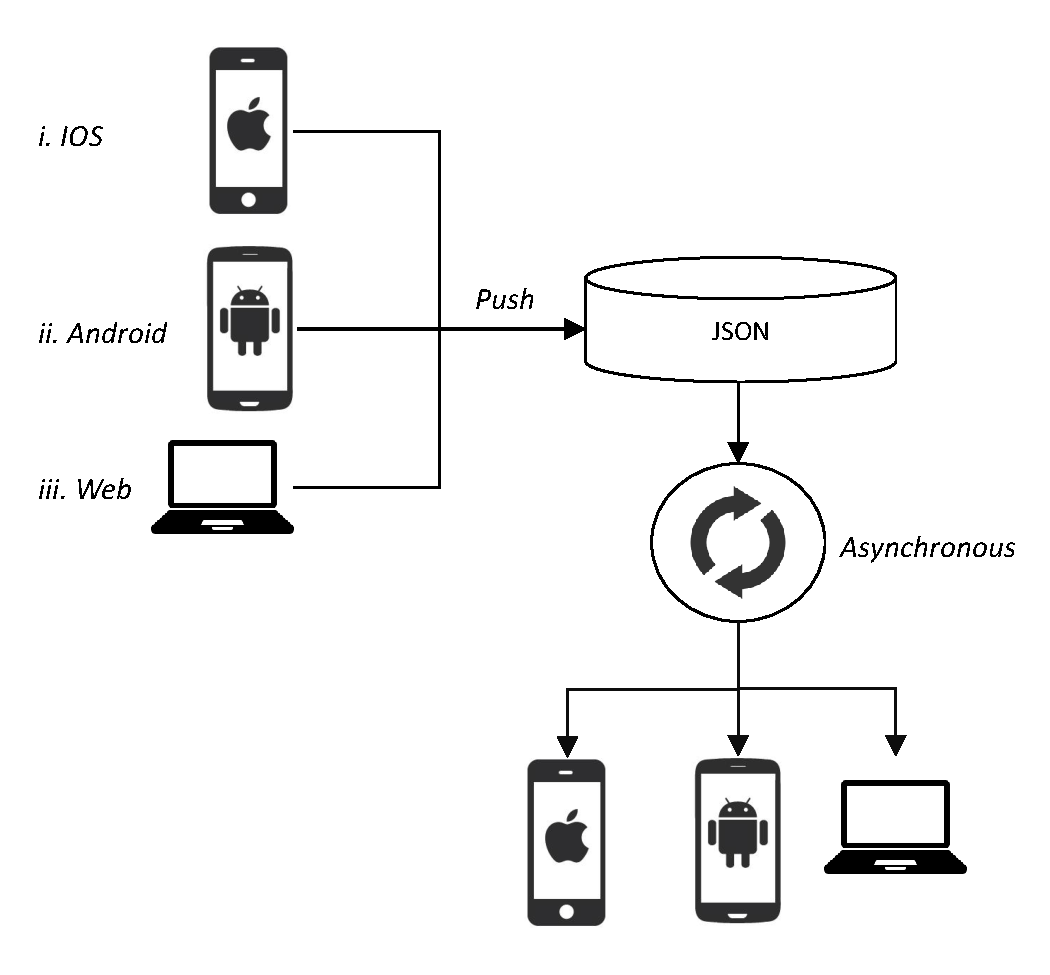
\includegraphics[width=0.6\textwidth]{figs/Architecture}
	\caption{Tasks platforms}
	\label{fig:Architecture}
\end{figure}


\subsection{Database and Back-end}

As earlier stated, we use Firebase as a back-end. This strategy implies to simplify the logic in the back-end and bestow more work to the clients. What we earn by this real fast reading updated than a common design, due to Firebase architecture that provides optimised sockets and a secure protocol.

Firebase consist of a real-time database with an API that allows to synchronise and store data in the cloud with multiple clients. It provides a client library that in our case allows the integration with Android,iOS and Web using Java, Swift and JavaScript respectively. Other services of Firebase as a platform is the storage, hosting (which support static files such as CSS, HTML, media and JavaScript).  To sum-up, Firebase plays a role as a real-time back-end, suitable for scalable applications.

Other interesting characteristic of Firebase is the authentication service, which support social login providers, such as Facebook, GitHub, Google, etc. Another brilliant feature that we used a lot for testing is that we could see in real time the modification of the data. Looking green when new nodes were added, yellow when modified and red when removed. In addition, the crash reporting, as well the analytics tools, caught our attention for two main reasons: i) the possibility to extract information in the future to make more friendly the application (e.g. with performance measures like the average time in the application), and ii) the possibility to test improvements and track changes, with for example A/B tests.

JSON (JavaScript Object Notation) is a lightweight data inter-change format, easier to generate for machines. It is based on i) a set of \textbf{key} and \textbf{value} duple (i.e. an object), and ii) an ordered list of values (i.e. can be string, number, array or even another object) ~\cite{1sejkfhs}. JSON is more lightweight than XML and thus is preferable for web applications because newcomers prefer to handle JSON instead of XML because of the lack of verbosity and readability. Also ~\cite{1sejkfhs} it includes a comparison between the advantages of JSON vs XML.

The following Figure ~\ref{fig:database} presents the structure of the designed database. The idea behind this structure is to prioritise the reading speeds, so messages can be transmitted faster (thus, we duplicate in some cases the data across the tables). That is a strange thing for users that commonly work with relational databases, as a lot of the information tends to be duplicated and not normalised. However, because Firebase is very lightweight, the repetition is not a problem.

\begin{figure}[ht]
\centering
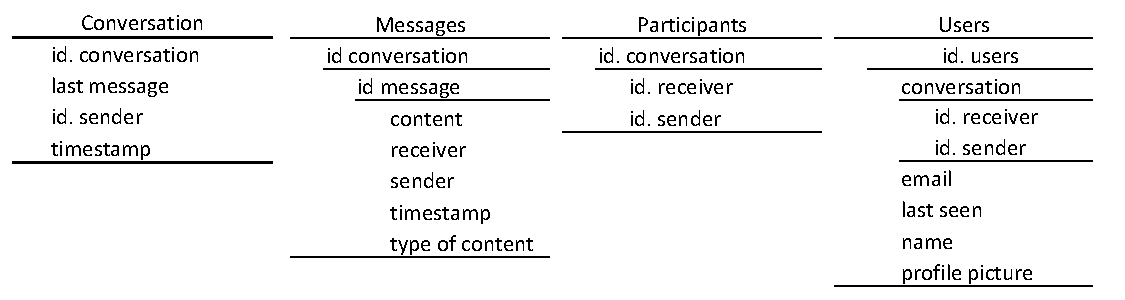
\includegraphics[width=1\textwidth]{figs/database}
	\caption{Database structure}
	\label{fig:database}
\end{figure}

As a comparison exercise, we based our decision starting on a classic design of a relational database, which is showed in Figure ~\ref{fig:rdatabase}. Then, we migrated the design to JSON based on the suggestions that we found online and in the main Firebase docs, this is to optimise its value and allow us to add security and validation rules.

\begin{figure}[ht]
\centering
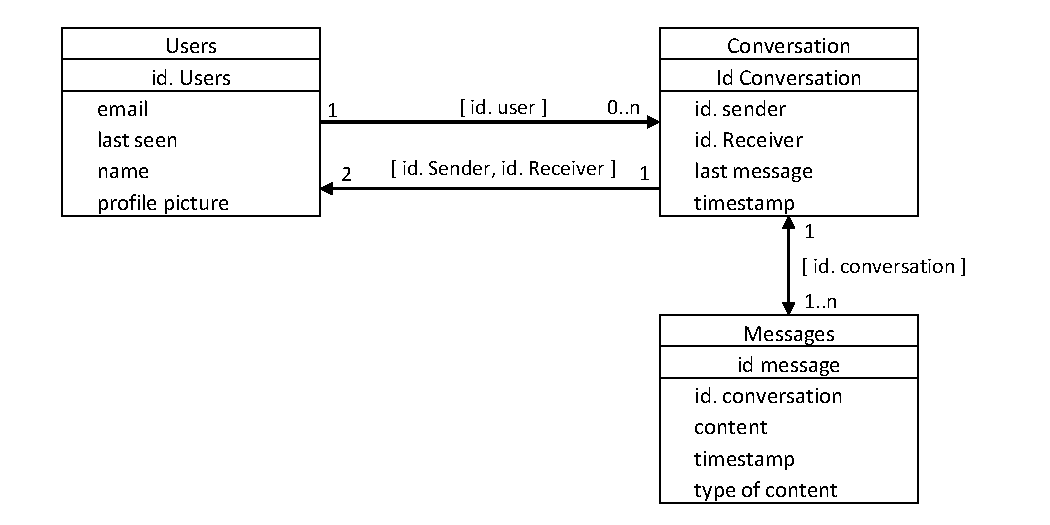
\includegraphics[width=0.9\textwidth]{figs/relationaldatabase}
	\caption{Relational Database initial structure}
	\label{fig:rdatabase}
\end{figure}

The design specified in Figure ~\ref{fig:rdatabase} was also proposed considered the following interaction across the tables, based on three fundamental features: i) sign in, ii) sign up and iii) send messages.  In the case of sign in, the user information last seen field is updated each time. For the Signing up, the \textbf{uid} created by Firebase Auth System is used to create a new user, with the basic information (i.e. id, name, email, and profile picture). Finally, send messages is the most interactive functionality, which works by recovering a conversation id or creating a new id in case there isn't a conversation between two participants available. Furthermore creates a new message which is appended to the respective conversation. To make the query of information easier, the participants table keeps the conversation id, with their respective users id with a value of true in case it exists in that table. We use id.receiver and id.sender for simplicity, however the real sender and receiver properties are shown on the messages dictionary.

\begin{figure}[ht]
\centering
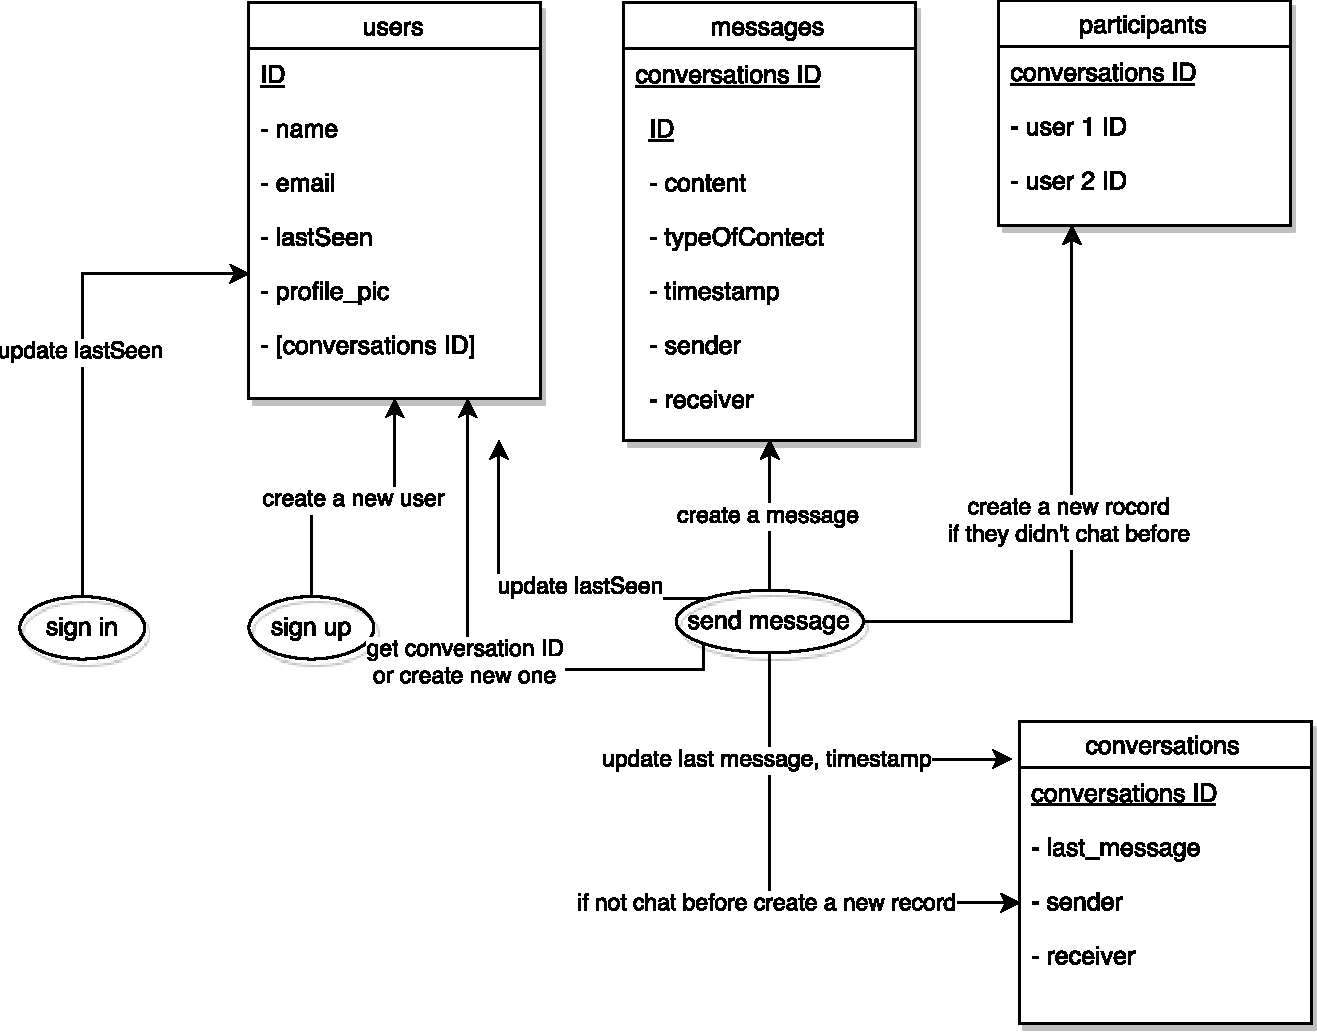
\includegraphics[width=0.8\textwidth]{figs/database_interaction}
	\caption{Database Interactions}
	\label{fig:rdatabaseinter}
\end{figure}


The next section gives more details about the implementation of each specific client. However, the three previously described functionalities and interaction with the database hold for all of them. 
